\documentclass{report}
\usepackage{fancyhdr} % Required for custom headers
\usepackage{lastpage} % Required to determine the last page for the footer
\usepackage{extramarks} % Required for headers and footers
\usepackage{graphicx} % Required to insert images
%\usepackage{lipsum} % Used for inserting dummy 'Lorem ipsum' text into the template
\usepackage{amsmath}
\usepackage{graphicx} 
\usepackage{float}
%\usepackage{amsfont}
%\usepackage{amssymb}

\usepackage{multicol}
% Margins
\topmargin=-0.5in
\evensidemargin=0in
\oddsidemargin=-0.5in
\textwidth=7.5in
\textheight=9.0in
\headsep=0.25in 


\pagestyle{fancy}

%\rhead{\textbf{Marshall's Recipes}} % Top right header
%\lhead{\textbf{Curry Stir Fry}}
%\chead{ }
%\title{Curry Stir Fry}

\begin{document}
%\vspace{8mm}
%\textbf{PRELIMINARIES:}


\bigskip

\bigskip

\begin{multicols}{2}
\textbf{Ingredients}
\begin{itemize}
\item $1\frac{1}{2}$ cup rolled oats \quad (450 kCal / 15 gP / 8 gF / 81 gC)
\item $1\frac{1}{2}$ cup oat milk \quad (195 kCal / 6 gP / 5 gF / 23 gC) 
\item $\frac{3}{4}$ cup of vanilla yogurt \newline (80 kCal / 5 gP / 0 gF / 15 gC) 
\item 3 tbsp. maple syrup \quad (165 kCal / 0 gP / 0 gF / 41 gC)
\item 3 tbsp. chia seeds \quad (210 kCal / 9 gP / 15 gF / 3 gC)
\item 3 tbsp. sliced almonds \quad (90 kCal / 3 gP / 8 gF / 3 gC) 
\item 2 small-medium apples, chopped \newline (190 kCal / 2 gP / 0 gF / 50 gC)
\item $1\frac{1}{2}$ tsp. ground cinnamon




\end{itemize}


\columnbreak
\textbf{Procedure:}
\medskip


\begin{enumerate}
\item Using 3 clean mason jars, put $\frac{1}{2}$ cup of oats in each jar, then $\frac{1}{4}$ cup yogurt in each jar. 

\item Next, add in $\frac{1}{2}$ cup oat milk and 1 tbsp. maple syrup to each jar. Add $\frac{1}{2}$ tsp. cinnamon to each jar, stir, and top with about $\frac{1}{3}$rd of the chopped apples. 

\item Finish by adding 1 tbsp. chia seeds and 1 tbsp. sliced almonds to the top and sealing. Refrigerate overnight.

\begin{table}[H]
  \begin{center}
    \caption{Macro totals}
    \label{tab:table1}
    \begin{tabular}{c|c|c|c} % <-- Alignments: 1st column left, 2nd middle and 3rd right, with vertical lines in between
      \textbf{Calories} & \textbf{Protein} & \textbf{Fat} & \textbf{Carbs}\\
      \hline
      1,380 kCal & 40 g & 36 g & 216 g\\
    \end{tabular}
  \end{center}
\end{table}
 
\end{enumerate}
\end{multicols}




%\begin{center}
%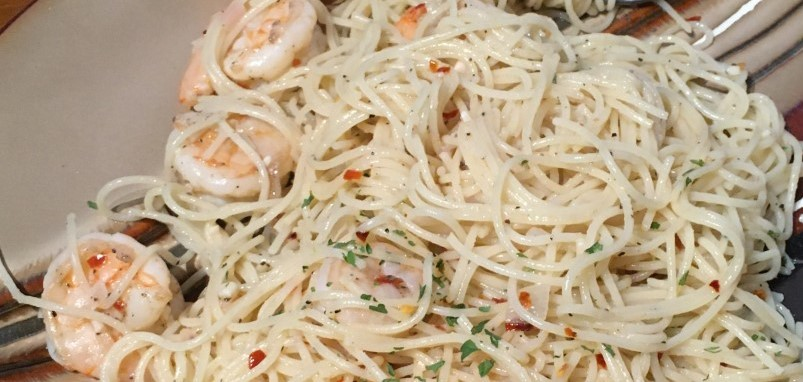
\includegraphics[scale=0.65]{Pasta/Shrimp Scampi/Shrimp Scampi.jpg}
%\end{center}


\end{document}